

\tikzset{every picture/.style={line width=0.75pt}} %set default line width to 0.75pt        

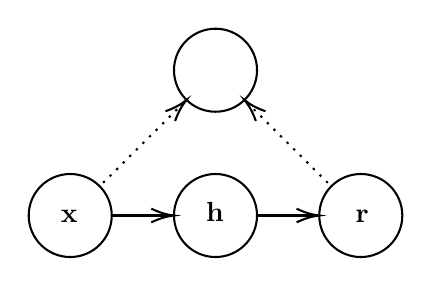
\begin{tikzpicture}[x=0.75pt,y=0.75pt,yscale=-1,xscale=1]
%uncomment if require: \path (0,148); %set diagram left start at 0, and has height of 148

%Shape: Boxed Line [id:dp8923577175434361] 
\draw  [dash pattern={on 0.84pt off 2.51pt}]  (70,110) -- (124.54,55.81) ;
\draw [shift={(125.96,54.4)}, rotate = 495.18] [color={rgb, 255:red, 0; green, 0; blue, 0 }  ][line width=0.75]    (10.93,-3.29) .. controls (6.95,-1.4) and (3.31,-0.3) .. (0,0) .. controls (3.31,0.3) and (6.95,1.4) .. (10.93,3.29)   ;
%Shape: Boxed Line [id:dp9855569745062982] 
\draw  [dash pattern={on 0.84pt off 2.51pt}]  (209.96,110) -- (155.42,55.81) ;
\draw [shift={(154,54.4)}, rotate = 404.82] [color={rgb, 255:red, 0; green, 0; blue, 0 }  ][line width=0.75]    (10.93,-3.29) .. controls (6.95,-1.4) and (3.31,-0.3) .. (0,0) .. controls (3.31,0.3) and (6.95,1.4) .. (10.93,3.29)   ;
%Shape: Circle [id:dp5965402013258883] 
\draw   (120,110) .. controls (120,98.95) and (128.95,90) .. (140,90) .. controls (151.05,90) and (160,98.95) .. (160,110) .. controls (160,121.05) and (151.05,130) .. (140,130) .. controls (128.95,130) and (120,121.05) .. (120,110) -- cycle ;
%Shape: Circle [id:dp24273838994586128] 
\draw  [fill={rgb, 255:red, 255; green, 255; blue, 255 }  ,fill opacity=1 ] (50,110) .. controls (50,98.95) and (58.95,90) .. (70,90) .. controls (81.05,90) and (90,98.95) .. (90,110) .. controls (90,121.05) and (81.05,130) .. (70,130) .. controls (58.95,130) and (50,121.05) .. (50,110) -- cycle ;
%Shape: Circle [id:dp07818860842911124] 
\draw  [fill={rgb, 255:red, 255; green, 255; blue, 255 }  ,fill opacity=1 ] (190,110) .. controls (190,98.95) and (198.95,90) .. (210,90) .. controls (221.05,90) and (230,98.95) .. (230,110) .. controls (230,121.05) and (221.05,130) .. (210,130) .. controls (198.95,130) and (190,121.05) .. (190,110) -- cycle ;
%Shape: Circle [id:dp6286535373530038] 
\draw   (120,40) .. controls (120,28.95) and (128.95,20) .. (140,20) .. controls (151.05,20) and (160,28.95) .. (160,40) .. controls (160,51.05) and (151.05,60) .. (140,60) .. controls (128.95,60) and (120,51.05) .. (120,40) -- cycle ;
%Straight Lines [id:da3987012470307014] 
\draw    (90,110) -- (118,110) ;
\draw [shift={(120,110)}, rotate = 180] [color={rgb, 255:red, 0; green, 0; blue, 0 }  ][line width=0.75]    (10.93,-3.29) .. controls (6.95,-1.4) and (3.31,-0.3) .. (0,0) .. controls (3.31,0.3) and (6.95,1.4) .. (10.93,3.29)   ;
%Straight Lines [id:da5505317995787229] 
\draw    (160,110) -- (188,110) ;
\draw [shift={(190,110)}, rotate = 180] [color={rgb, 255:red, 0; green, 0; blue, 0 }  ][line width=0.75]    (10.93,-3.29) .. controls (6.95,-1.4) and (3.31,-0.3) .. (0,0) .. controls (3.31,0.3) and (6.95,1.4) .. (10.93,3.29)   ;

% Text Node
\draw (134,102) node [anchor=north west][inner sep=0.75pt]    {$\mathbf{h}$};
% Text Node
\draw (64,106) node [anchor=north west][inner sep=0.75pt]    {$\mathbf{x}$};
% Text Node
\draw (206,106) node [anchor=north west][inner sep=0.75pt]    {$\mathbf{r}$};
% Text Node
\draw (133,33) node [anchor=north west][inner sep=0.75pt]    {$\Loss$};


\end{tikzpicture}